\documentclass[compress]{beamer}
\usepackage{ifthen,verbatim,ulem}

\title{Status of Muon Alignment: HIP Algorithm}
\author{Jim Pivarski, Alexei Safonov, K\'aroly Banicz$^*$}
\institute{Texas A\&M University, $^*$FermiLab}
\date{14 May, 2008}

\newcommand{\isnote}{}
\xdefinecolor{lightyellow}{rgb}{1.,1.,0.25}
\xdefinecolor{darkblue}{rgb}{0.1,0.1,0.7}

%% Uncomment this to get annotations
%% \def\notes{\addtocounter{page}{-1}
%%            \renewcommand{\isnote}{*}
%% 	   \beamertemplateshadingbackground{lightyellow}{white}
%%            \begin{frame}
%%            \frametitle{Notes for the previous page (page \insertpagenumber)}
%%            \itemize}
%% \def\endnotes{\enditemize
%% 	      \end{frame}
%%               \beamertemplateshadingbackground{white}{white}
%%               \renewcommand{\isnote}{}}

%% Uncomment this to not get annotations
\def\notes{\comment}
\def\endnotes{\endcomment}

\setbeamertemplate{navigation symbols}{}
\setbeamertemplate{headline}{\mbox{ } \hfill
\begin{minipage}{5.5 cm}
\vspace{-0.75 cm} \small
\end{minipage} \hfill
\begin{minipage}{4.5 cm}
\vspace{-0.75 cm} \small
\begin{flushright}
\ifthenelse{\equal{\insertpagenumber}{1}}{}{Jim Pivarski \hspace{0.2 cm} \insertpagenumber\isnote/\pageref{numpages}}
\end{flushright}
\end{minipage}\mbox{\hspace{0.2 cm}}\includegraphics[height=1 cm]{../cmslogo} \hspace{0.1 cm} \includegraphics[height=1 cm]{../tamulogo} \hspace{0.01 cm} \vspace{-1.05 cm}}

\begin{document}
\frame{\titlepage}

%% \begin{notes}
%% \item This is the annotated version of my talk.
%% \item If you want the version that I am presenting, download the one
%% labeled ``slides'' on Indico (or just ignore these yellow pages).
%% \item The annotated version is provided for extra detail and a written
%% record of comments that I intend to make orally.
%% \item Yellow notes refer to the content on the {\it previous} page.
%% \item All other slides are identical for the two versions.
%% \end{notes}

\begin{frame}
\frametitle{Status on one slide}
\begin{itemize}\setlength{\itemsep}{0.25 cm}
\item Until this morning, muon alignment samples were inaccessible (except by CRAB)
\item Thanks to effort of production team, framework group, a work-around has been implemented
\item Work-around solves all problems except application of $p_T$ cut in alignment job
\begin{itemize}\setlength{\itemsep}{0.1 cm}
\item Needed to optimize alignment quality
\item Completed an alignment walk-through without the $p_T$ cut
\item Copying samples to a private skim seems to solve this problem (copy in progress)
\end{itemize}
\item Also applied a provisional tracker alignment (alignment job \sout{in~progress} just finished)
\item Strange peak in barrel residuals: will study
\item Baseline alignment will very likely be ready for Friday
\end{itemize}
%% \hspace{-0.83 cm} \textcolor{darkblue}{\Large Outline2}
\end{frame}

\begin{frame}
\frametitle{Barrel \only<1>{aligned positions}\only<2>{track residuals} (low $p_T$!)}

\only<1>{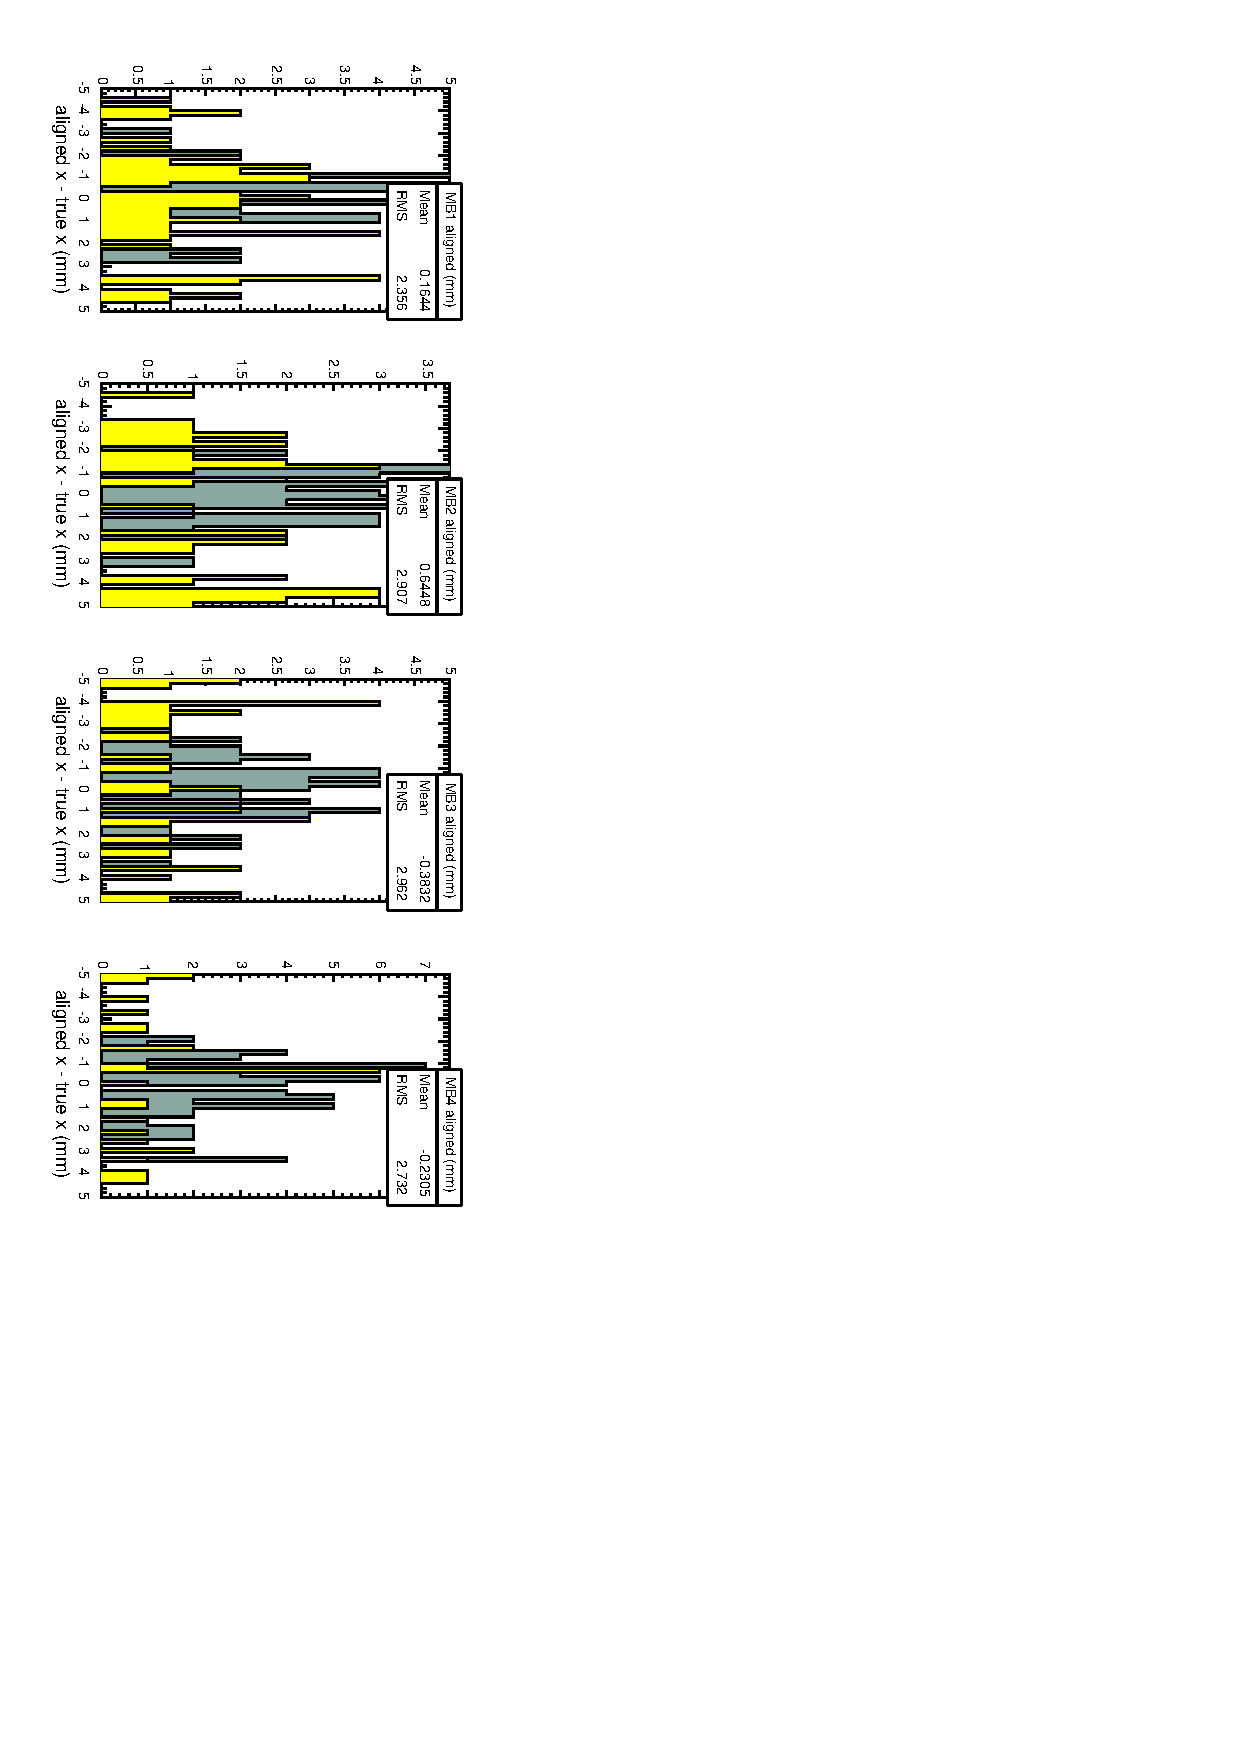
\includegraphics[height=\linewidth, angle=90]{baseline_MuonPT5_barrel.pdf}}
\only<2>{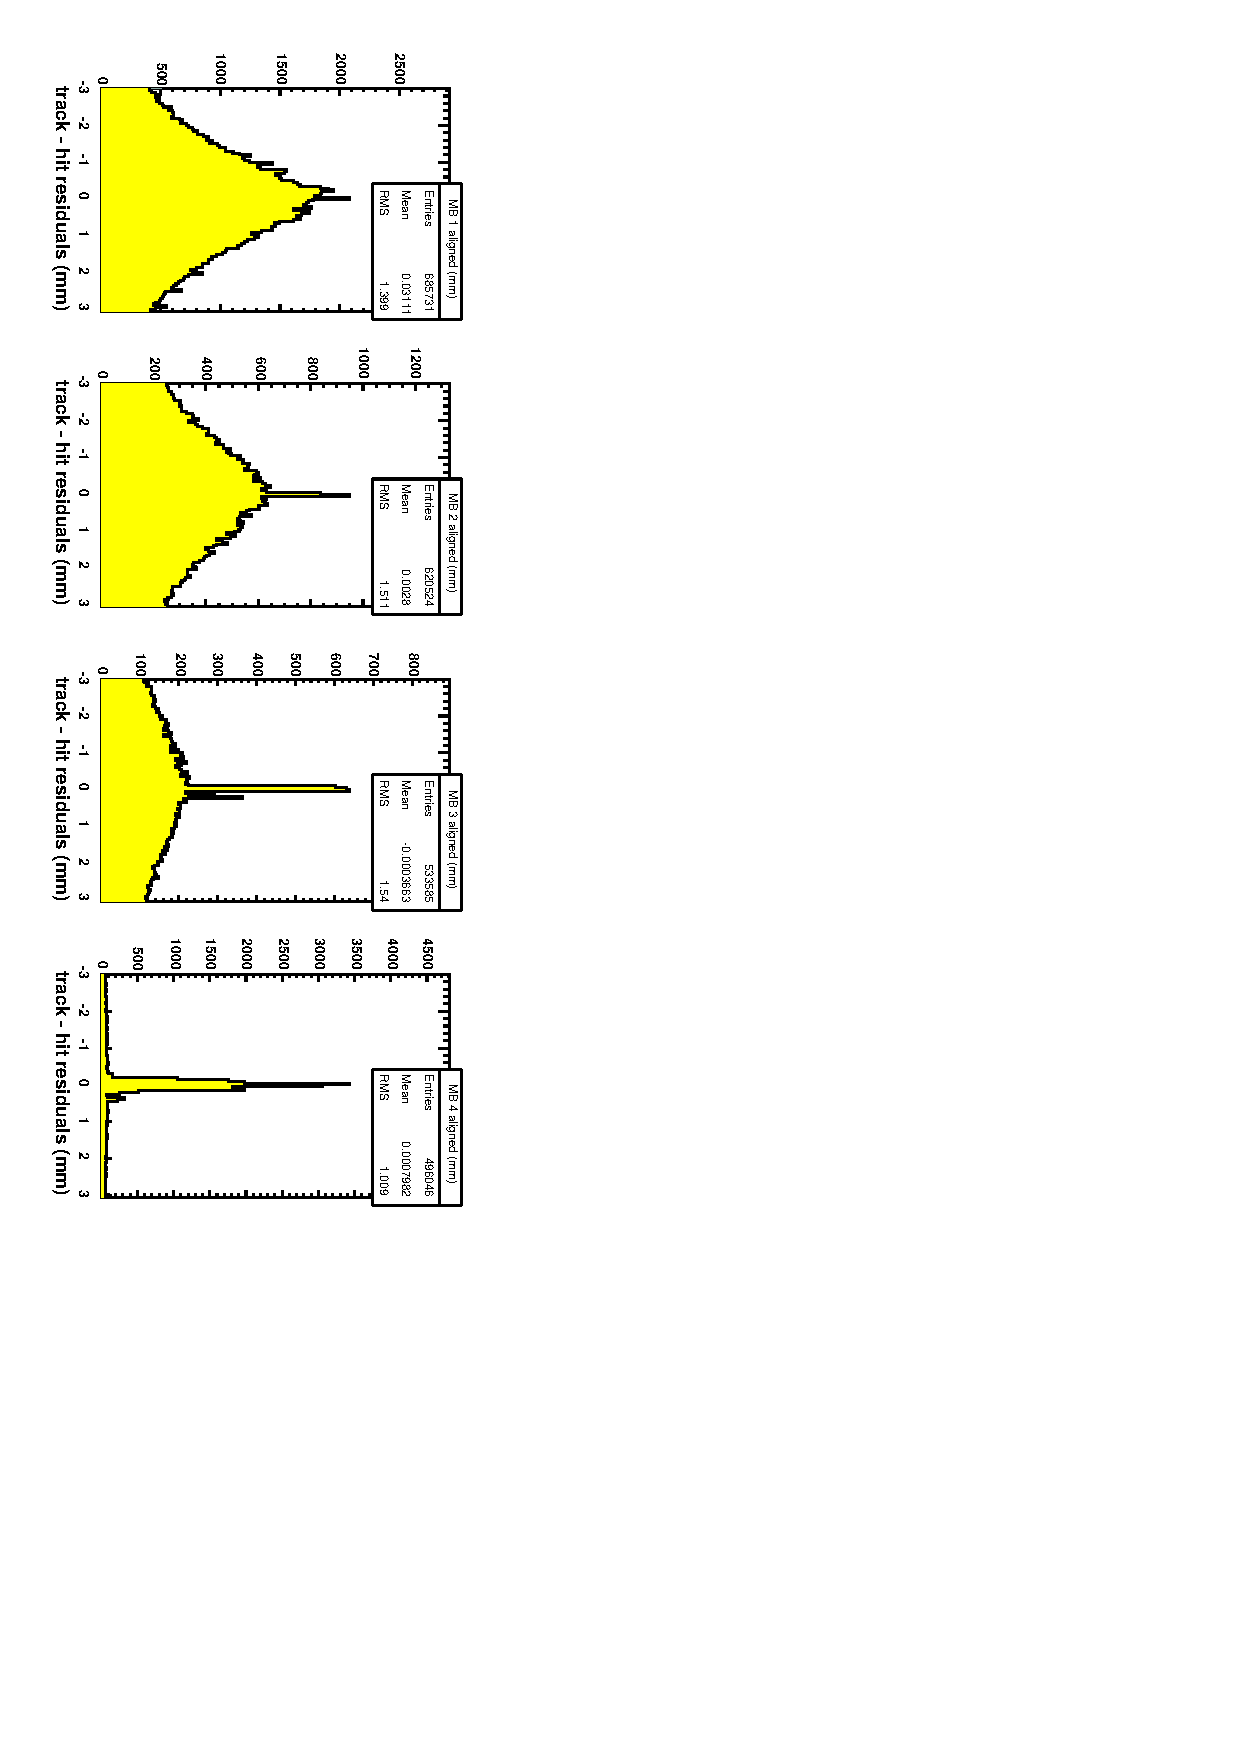
\includegraphics[height=\linewidth, angle=90]{baseline_MuonPT5_barrelresid.pdf}}

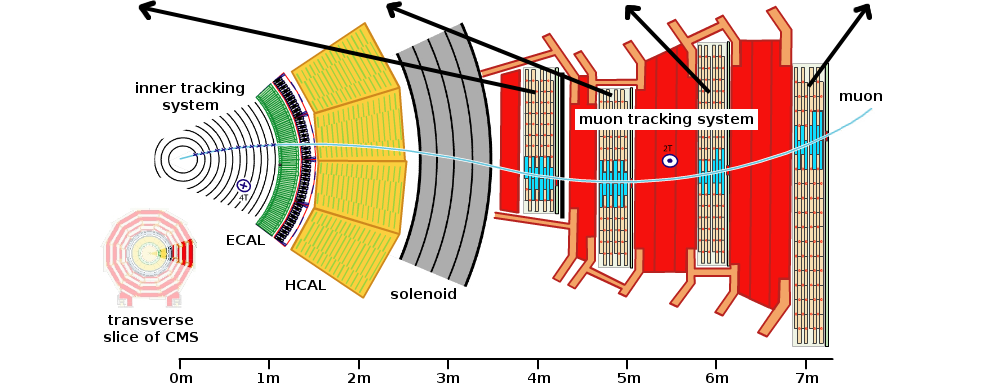
\includegraphics[width=\linewidth]{cms_slice.png}
\end{frame}

\begin{frame}
\frametitle{Endcap \only<1>{aligned positions}\only<2>{track residuals} (low $p_T$!)}

\begin{columns}
\column{0.35\linewidth}
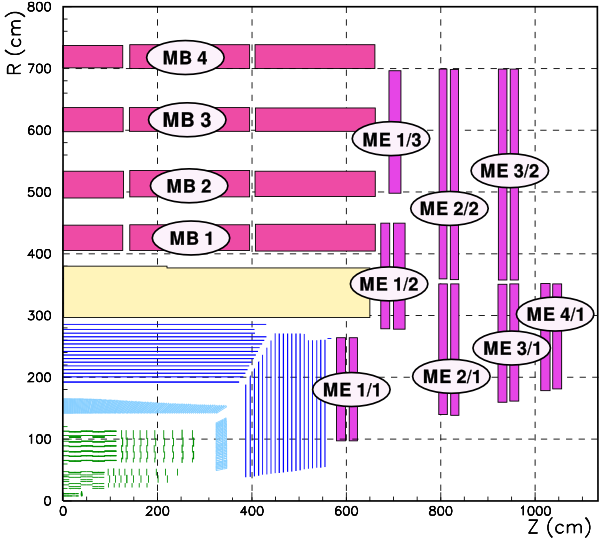
\includegraphics[width=\linewidth]{muon_system.png}
\column{0.8\linewidth}
\only<1>{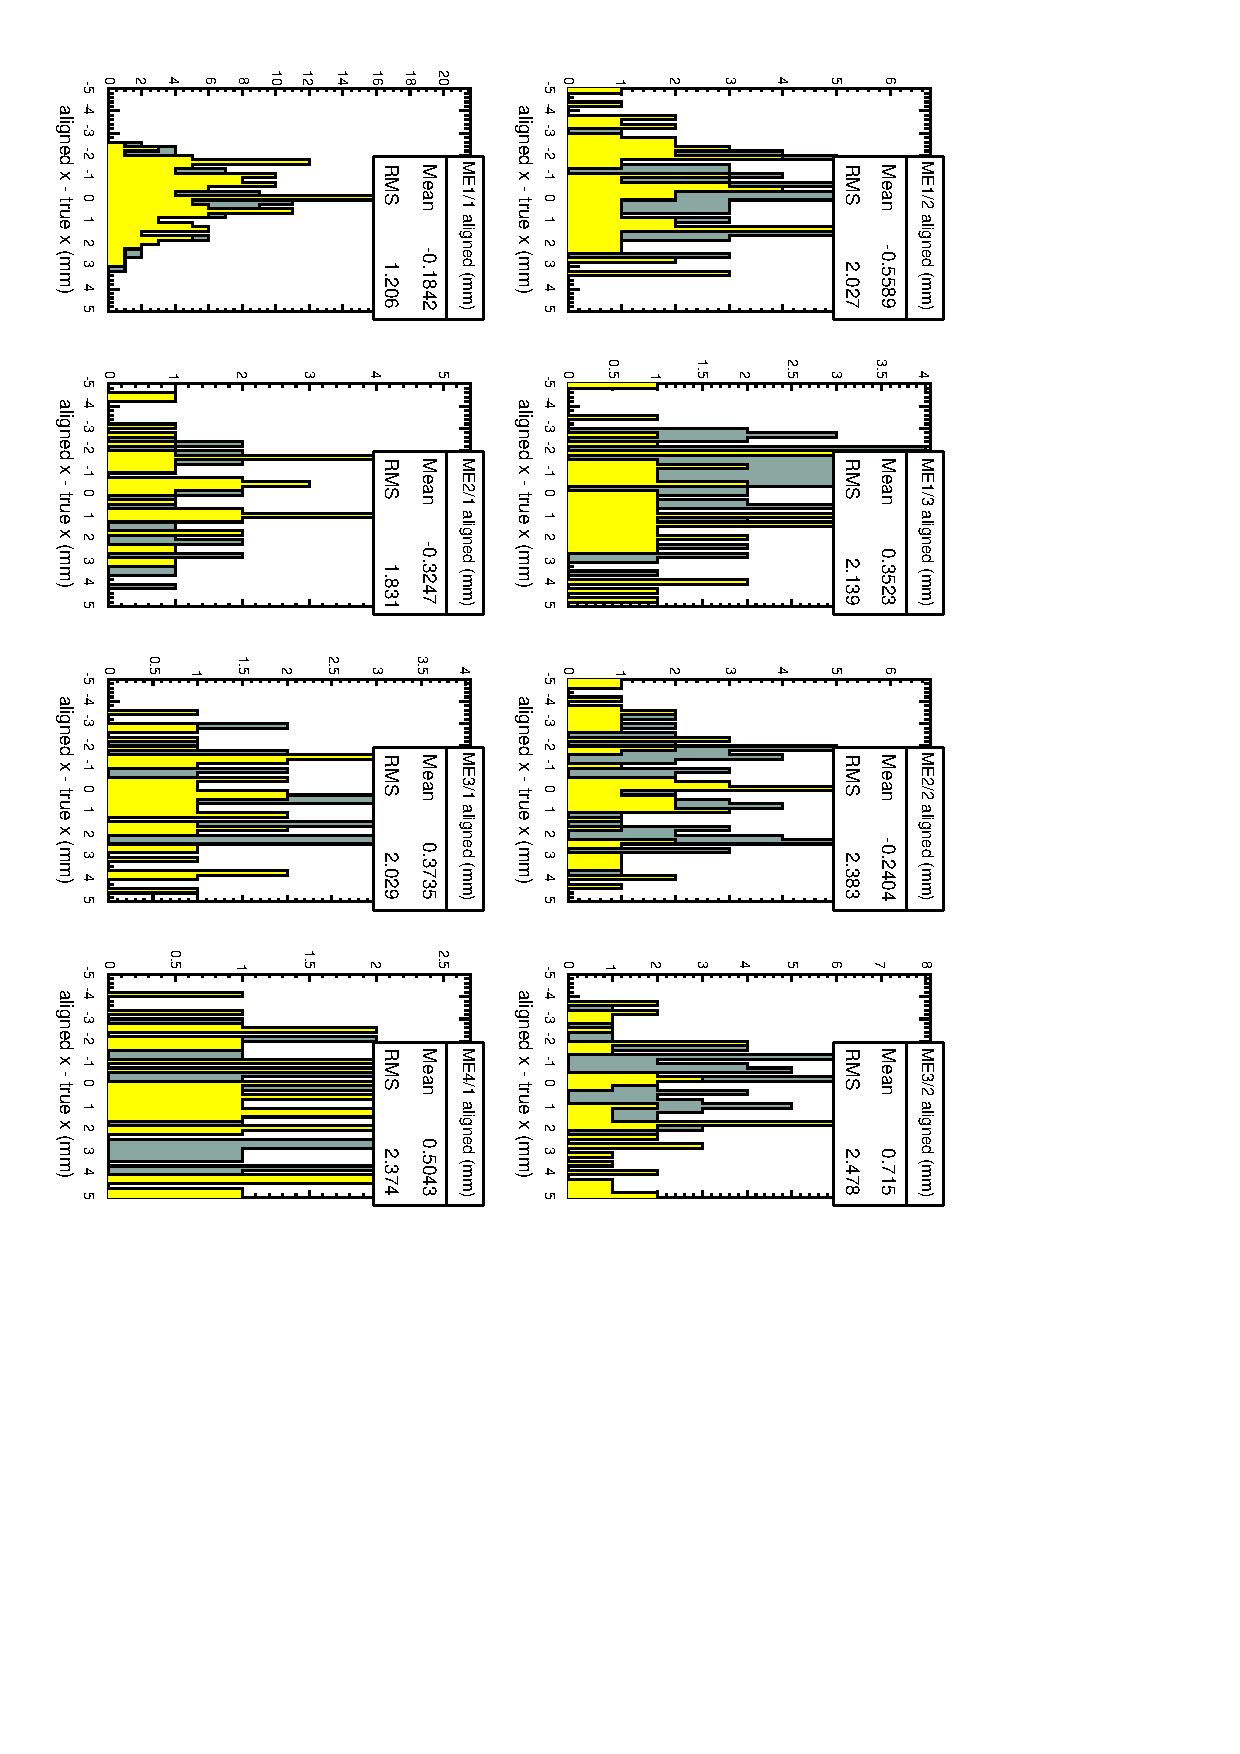
\includegraphics[height=\linewidth, angle=90]{baseline_MuonPT5_endcap.pdf}}
\only<2>{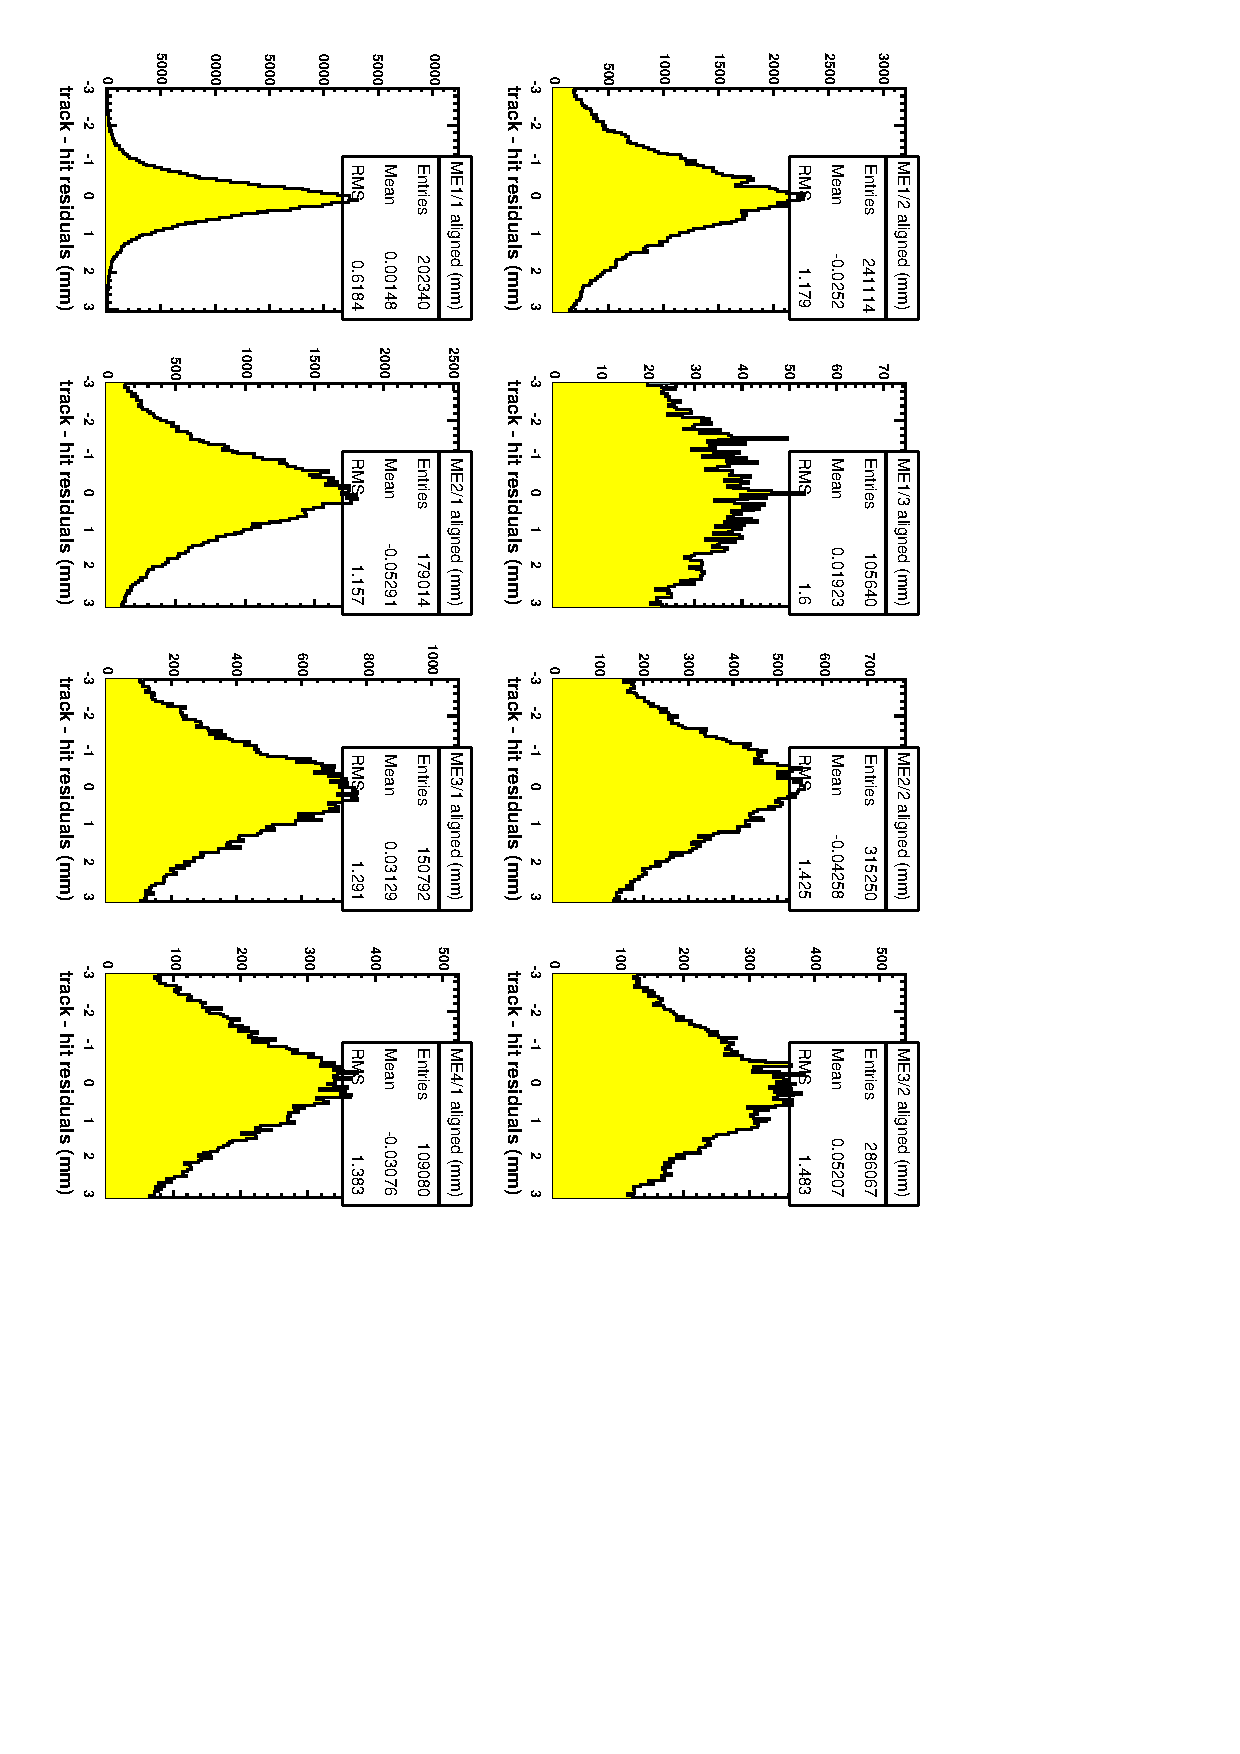
\includegraphics[height=\linewidth, angle=90]{baseline_MuonPT5_endcapresid.pdf}}
\end{columns}

\end{frame}




%% \section*{First section}
%% \begin{frame}
%% \begin{center}
%% \Huge \textcolor{blue}{First section}
%% \end{center}
%% \end{frame}

\begin{frame}
\label{numpages}
\end{frame}

\end{document}
